
\chapter{Lab 1: Monte Carlo Statistical Analysis}
\label{chap:lab_qmc_statistics}


\section{Topics covered in this Lab} 

This lab focuses on the basics of analyzing data from Monte Carlo (MC)
calculations.  In this lab, participants will use data from
VMC calculations of a simple one-electron system with an analytically soluble
system (the ground state of the hydrogen atom) to understand how to interpret a
MC situation.  Most of these analyses will also carry over to diffusion Monte
Carlo (DMC) simulations.  Topics covered include:
\begin{itemize}
  \item{averaging Monte Carlo variables}
  \item{the statisical error bar of mean values}
  \item{effects of autocorrelation and variance on the error bar}
  \item{the relationship between Monte Carlo timestep and autocorrelation}
  \item{the use of blocking to reduce autocorrelation}
  \item{the significance of the acceptance ratio}
  \item{the significance of the sample size}
  \item{how to determine whether a Monte Carlo run was successful}
  \item{the relationship between wavefunction quality and variance}
  \item{gauging the efficiency of Monte Carlo runs}
  \item{the cost of scaling up to larger system sizes}
\end{itemize}


\hide{
\subsection{How to get the most out of this lab}
Be sure to practice using the various flags in the qmca tool to analyze the
data.  Although some features are not yet implemented, this will get you used
to seeing how the values in the data files produce the averages, which are the
ultimate result of the MC simulations.
}

\section{Lab directories and files}

\footnotesize
\begin{verbatim}
labs/lab1_qmc_statistics/
│
├── atom                              - H atom VMC calculation
│   ├── H.s000.scalar.dat                - H atom VMC data 
│   └── H.xml                            - H atom VMC input file
│
├── autocorrelation                   - varying autocorrelation
│   ├── H.dat                            - data for gnuplot
│   ├── H.plt                            - gnuplot for time step vs. E_L, tau_c
│   ├── H.s000.scalar.dat                - H atom VMC data: time step = 10 
│   ├── H.s001.scalar.dat                - H atom VMC data: time step =  5 
│   ├── H.s002.scalar.dat                - H atom VMC data: time step =  2 
│   ├── H.s003.scalar.dat                - H atom VMC data: time step =  1 
│   ├── H.s004.scalar.dat                - H atom VMC data: time step =  0.5
│   ├── H.s005.scalar.dat                - H atom VMC data: time step =  0.2
│   ├── H.s006.scalar.dat                - H atom VMC data: time step =  0.1
│   ├── H.s007.scalar.dat                - H atom VMC data: time step =  0.05 
│   ├── H.s008.scalar.dat                - H atom VMC data: time step =  0.02
│   ├── H.s009.scalar.dat                - H atom VMC data: time step =  0.01
│   ├── H.s010.scalar.dat                - H atom VMC data: time step =  0.005
│   ├── H.s011.scalar.dat                - H atom VMC data: time step =  0.002
│   ├── H.s012.scalar.dat                - H atom VMC data: time step =  0.001
│   ├── H.s013.scalar.dat                - H atom VMC data: time step =  0.0005
│   ├── H.s014.scalar.dat                - H atom VMC data: time step =  0.0002
│   ├── H.s015.scalar.dat                - H atom VMC data: time step =  0.0001
│   └── H.xml                            - H atom VMC input file
│
├── average                            - Python scripts for average/std. dev.
│   ├── average.py                         - average five E_L from H atom VMC
│   ├── stddev2.py                         - standard deviation using (E_L)^2
│   └── stddev.py                          - standard deviation around the mean
│
├── basis                              - varying basis set for orbitals
│   ├── H__exact.s000.scalar.dat           - H atom VMC data using STO basis
│   ├── H_STO-2G.s000.scalar.dat           - H atom VMC data using STO-2G basis
│   ├── H_STO-3G.s000.scalar.dat           - H atom VMC data using STO-3G basis
│   └── H_STO-6G.s000.scalar.dat           - H atom VMC data using STO-6G basis
│
├── blocking                           - varying block/step ratio
│   ├── H.dat                              - data for gnuplot
│   ├── H.plt                              - gnuplot for N_block vs. E, tau_c
│   ├── H.s000.scalar.dat                  - H atom VMC data 50000:1 blocks:steps
│   ├── H.s001.scalar.dat                  - "  "    "    "  25000:2 blocks:steps
│   ├── H.s002.scalar.dat                  - "  "    "    "  12500:4 blocks:steps
│   ├── H.s003.scalar.dat                  - "  "    "    "  6250: 8 blocks:steps
│   ├── H.s004.scalar.dat                  - "  "    "    "  3125:16 blocks:steps
│   ├── H.s005.scalar.dat                  - "  "    "    "  2500:20 blocks:steps
│   ├── H.s006.scalar.dat                  - "  "    "    "  1250:40 blocks:steps
│   ├── H.s007.scalar.dat                  - "  "    "    "  1000:50 blocks:steps
│   ├── H.s008.scalar.dat                  - "  "    "    "  500:100 blocks:steps
│   ├── H.s009.scalar.dat                  - "  "    "    "  250:200 blocks:steps
│   ├── H.s010.scalar.dat                  - "  "    "    "  125:400 blocks:steps
│   ├── H.s011.scalar.dat                  - "  "    "    "  100:500 blocks:steps
│   ├── H.s012.scalar.dat                  - "  "    "    "  50:1000 blocks:steps
│   ├── H.s013.scalar.dat                  - "  "    "    "  40:1250 blocks:steps
│   ├── H.s014.scalar.dat                  - "  "    "    "  20:2500 blocks:steps
│   ├── H.s015.scalar.dat                  - "  "    "    "  10:5000 blocks:steps
│   └── H.xml                             - H atom VMC input file
│
├── blocks                             -  varying total number of blocks
│   ├── H.dat                             - data for gnuplot
│   ├── H.plt                             - gnuplot for N_block vs. E
│   ├── H.s000.scalar.dat                 - H atom VMC data    500 blocks
│   ├── H.s001.scalar.dat                 - "  "    "    "    2000 blocks
│   ├── H.s002.scalar.dat                 - "  "    "    "    8000 blocks
│   ├── H.s003.scalar.dat                 - "  "    "    "   32000 blocks
│   ├── H.s004.scalar.dat                 - "  "    "    "  128000 blocks
│   └── H.xml                             - H atom VMC input file 
│
├── dimer                          - comparing no and simple Jastrow factor
│   ├── H2_STO___no_jastrow.s000.scalar.dat - H dimer VMC data without Jastrow
│   └── H2_STO_with_jastrow.s000.scalar.dat - H dimer VMC data with Jastrow
│
├──  docs                               - documentation
│   ├──  Lab_1_MC_Analysis.pdf             - this document
│   └──  Lab_1_Slides.pdf                  - slides presented in the lab
│
├── nodes                              - varying number of computing nodes
│   ├──  H.dat                             - data for gnuplot
│   ├──  H.plt                             - gnuplot for N_node vs. E
│   ├──  H.s000.scalar.dat                 - H atom VMC data with  32 nodes
│   ├──  H.s001.scalar.dat                 - H atom VMC data with 128 nodes
│   └──  H.s002.scalar.dat                 - H atom VMC data with 512 nodes
│
├── problematic                        - problematic VMC run
│   └──  H.s000.scalar.dat                 - H atom VMC data with a problem
│
└── size                                - scaling with number of particles
    ├──  01________H.s000.scalar.dat       - H atom VMC data
    ├──  02_______H2.s000.scalar.dat       - H dimer "   "
    ├──  06________C.s000.scalar.dat       - C atom  "   "
    ├──  10______CH4.s000.scalar.dat       - methane "   "
    ├──  12_______C2.s000.scalar.dat       - C dimer "   "
    ├──  16_____C2H4.s000.scalar.dat       - ethene  " 
    ├──  18___CH4CH4.s000.scalar.dat       - methane dimer VMC data
    ├──  32_C2H4C2H4.s000.scalar.dat       - ethene dimer   "   "
    ├──  nelectron_tcpu.dat                - data for gnuplot
    └──  Nelectron_tCPU.plt                - gnuplot for N_elec vs. t_CPU
\end{verbatim}
\normalsize

\section{Atomic units} 

QMCPACK operates in Hartree atomic units to reduce the
number of factors in the Schr\"odinger equation.  Thus, the unit of length is
the bohr (5.291772 $\times 10^{-11}$ m = 0.529177 \AA); the unit of energy is
the hartree (4.359744 $\times 10^{-18}$ J = 27.211385 eV).  The energy of the
ground state of the hydrogen atom in these units is -0.5 hartrees.


%\section{Monte Carlo data analysis:\newline average, error bars, variance}

\section{Reviewing statistics}
\label{sec:review}

We will practice taking the average (mean) and standard deviation of some Monte
Carlo data by hand to review the basic definitions.

Enter Python's command line by typing \textbf{python [Enter]}.
You will see a prompt ``\textgreater\textgreater\textgreater''.

The mean of a data set is given by:
\begin{align}
  \overline{x} = \frac{1}{N}\sum_{i=1}^{N} x_i
\end{align}

To calculate the average of five local energies from a MC calculation of the
ground state of an electron in the hydrogen atom, input (truncate at the
thousandths place if you cannot copy and paste; script versions are also
available in the \texttt{average} directory): 

\begin{lstlisting}[style=SHELL]
(
(-0.45298911858) + 
(-0.45481953564) + 
(-0.48066105923) + 
(-0.47316713469) + 
(-0.46204733302)
)/5.
\end{lstlisting} 

Then, press \textbf{[Enter]} to get:

\begin{shade}
>>> ((-0.45298911858) + (-0.45481953564) + (-0.48066105923) + 
(-0.47316713469) + (-0.4620473302))/5.  
-0.46473683566800006
\end{shade}

To understand the significance of the mean, we also need the standard deviation
around the mean of the data (also called the error bar), given by:

\begin{align}
  \sigma = \sqrt{\frac{1}{N(N-1)}\sum_{i=1}^{N} ({x_i} - \overline{x})^2}
\end{align}

To calculate the standard deviation around the mean (-0.464736835668) of these
five data points, put in: 

\begin{lstlisting}[style=SHELL]
( (1./(5.*(5.-1.))) * ( 
(-0.45298911858-(-0.464736835668))**2 + \\
(-0.45481953564-(-0.464736835668))**2 + 
(-0.48066105923-(-0.464736835668))**2 + 
(-0.47316713469-(-0.464736835668))**2 + 
(-0.46204733302-(-0.464736835668))**2 ) 
)**0.5
\end{lstlisting} 

Then, press \textbf{[Enter]} to get:

\begin{shade}
>>> ( (1./(5.*(5.-1.))) * ( (-0.45298911858-(-0.464736835668))**2 +
(-0.45481953564-(-0.464736835668))**2 + (-0.48066105923-(-0.464736835668))**2 + 
(-0.47316713469-(-0.464736835668))**2 + (-0.46204733302-(-0.464736835668))**2 
) )**0.5
0.0053303187464332066
\end{shade}

Thus, we might report this data as having a value -0.465 +/- 0.005 hartrees.
This calculation of the standard deviation assumes that the average for this
data is fixed, but we may continually add Monte Carlo samples to the data so it
is better to use an estimate of the error bar that does not rely on the overall
average.  Such an estimate is given by:

\begin{align}
  \tilde{\sigma} = \sqrt{\frac{1}{N-1}\sum_{i=1}^{N} \left[{(x^2)}_i - ({x_i})^2\right]}
\end{align}

To calculate the standard deviation with this formula, input the following,
which includes the square of the local energy calculated with each
corresponding local energy:

\begin{lstlisting}[style=SHELL]
( (1./(5.-1.)) * ( 
(0.60984565298-(-0.45298911858)**2) + \\
(0.61641291630-(-0.45481953564)**2) + 
(1.35860151160-(-0.48066105923)**2) + \\
(0.78720769003-(-0.47316713469)**2) + 
(0.56393677687-(-0.46204733302)**2) ) 
)**0.5
\end{lstlisting}

and press \textbf{[Enter]} to get:

\begin{shade}
>>> ((1./(5.-1.))*((0.60984565298-(-0.45298911858)**2)+ 
(0.61641291630-(-0.45481953564)**2)+(1.35860151160-(-0.48066105923)**2)+ 
(0.78720769003-(-0.47316713469)**2)+(0.56393677687-(-0.46204733302)**2))
)**0.5
0.84491636672906634
\end{shade}

This much larger standard deviation, acknowledging that the mean of this small
data set is not the average in the limit of infinite sampling more accurately,
reports the value of the local energy as -0.5 +/- 0.8 hartrees.

Type \textbf{quit()} and press \textbf{[Enter]} to exit the Python command line.

\section{Inspecting Monte Carlo data}
\label{sec:inspect_data} 

QMCPACK outputs data from MC calculations into files ending in scalar.dat.
Several quantities are calculated and written for each block of Monte Carlo
steps in successive columns to the right of the step index. 

Change directories to \texttt{atom}, and open the file ending in
scalar.dat with a text editor (e.g., \textbf{vi *.scalar.dat} or \textbf{emacs
*.scalar.dat}.  If possible, adjust the terminal so that lines do not wrap.
The data will begin as follows (broken into three groups to fit on this page):

\begin{shade}
#   index    LocalEnergy         LocalEnergy_sq      LocalPotential     ...
         0   -4.5298911858e-01    6.0984565298e-01   -1.1708693521e+00    
         1   -4.5481953564e-01    6.1641291630e-01   -1.1863425644e+00    
         2   -4.8066105923e-01    1.3586015116e+00   -1.1766446209e+00    
         3   -4.7316713469e-01    7.8720769003e-01   -1.1799481122e+00    
         4   -4.6204733302e-01    5.6393677687e-01   -1.1619244081e+00    
         5   -4.4313854290e-01    6.0831516179e-01   -1.2064503041e+00    
         6   -4.5064926960e-01    5.9891422196e-01   -1.1521370176e+00    
         7   -4.5687452611e-01    5.8139614676e-01   -1.1423627617e+00    
         8   -4.5018503739e-01    8.4147849706e-01   -1.1842075439e+00    
         9   -4.3862013841e-01    5.5477715836e-01   -1.2080979177e+00    
\end{shade}

The first line begins with a \#, indicating that this line does not contain MC
data but rather the labels of the columns.  After a blank line, the remaining
lines consist of the MC data.  The first column, labeled index, is an integer
indicating which block of MC data is on that line.  The second column contains
the quantity usually of greatest interest from the simulation, the local
energy.  Since this simulation did not use the exact ground state wave
function, it does not produce -0.5 hartrees as the local energy although the
value lies within about 10\%.  The value of the local energy fluctuates from
block to block and the closer the trial wave function is to the ground state,
the smaller these fluctuations will be.  The next column contains an important
ingredient in estimating the error in the MC average--the square of the local
energy--found by evaluating the square of the Hamiltonian.  

\begin{shade} 
...   Kinetic             Coulomb             BlockWeight        ... 
       7.1788023352e-01   -1.1708693521e+00    1.2800000000e+04   
       7.3152302871e-01   -1.1863425644e+00    1.2800000000e+04   
       6.9598356165e-01   -1.1766446209e+00    1.2800000000e+04   
       7.0678097751e-01   -1.1799481122e+00    1.2800000000e+04   
       6.9987707508e-01   -1.1619244081e+00    1.2800000000e+04   
       7.6331176120e-01   -1.2064503041e+00    1.2800000000e+04   
       7.0148774798e-01   -1.1521370176e+00    1.2800000000e+04   
       6.8548823555e-01   -1.1423627617e+00    1.2800000000e+04   
       7.3402250655e-01   -1.1842075439e+00    1.2800000000e+04   
       7.6947777925e-01   -1.2080979177e+00    1.2800000000e+04   
\end{shade}

The fourth column from the left consists of the values of the local potential
energy.  In this simulation, it is identical to the Coulomb potential
(contained in the sixth column) because the one electron in the simulation has
only the potential energy coming from its interaction with the nucleus.  In
many-electron simulations, the local potential energy contains contributions
from the electron-electron Coulomb interactions and the nuclear potential or
pseudopotential.  The fifth column contains the local kinetic energy value for
each MC block, obtained from the Laplacian of the wave function.  The sixth
column shows the local Coulomb interaction energy.  The seventh column displays
the weight each line of data has in the average (the weights are identical in
this simulation).   

\begin{shade} 
...    BlockCPU            AcceptRatio         
       6.0178991748e-03    9.8515625000e-01
       5.8323097461e-03    9.8562500000e-01
       5.8213412744e-03    9.8531250000e-01
       5.8330412549e-03    9.8828125000e-01
       5.8108362256e-03    9.8625000000e-01
       5.8254170264e-03    9.8625000000e-01
       5.8314813086e-03    9.8679687500e-01
       5.8258469971e-03    9.8726562500e-01
       5.8158433545e-03    9.8468750000e-01
       5.7959401123e-03    9.8539062500e-01
\end{shade}

The eighth column shows the CPU time (in seconds) to calculate the data in that
line.  The ninth column from the left contains the acceptance ratio (1 being
full acceptance) for Monte Carlo steps in that line's data.  Other than the
block weight, all quantities vary from line to line.

Exit the text editor (\textbf{[Esc] :q! [Enter]} in vi, \textbf{[Ctrl]-x [Ctrl]-c} in
emacs).

\section{Averaging quantities in the MC data}
\label{sec:averaging} 

QMCPACK includes the qmca Python tool to average quantities in the scalar.dat file (and
also the dmc.dat file of DMC simulations).  Without any flags, qmca will output
the average of each column with a quantity in the scalar.dat file as follows. 

Execute qmca by \textbf{qmca *.scalar.dat}, which for this data outputs:

\begin{shade}

H  series 0 
LocalEnergy           =          -0.45446 +/-          0.00057
Variance              =             0.529 +/-            0.018 
Kinetic               =            0.7366 +/-           0.0020
LocalPotential        =           -1.1910 +/-           0.0016
Coulomb               =           -1.1910 +/-           0.0016 
LocalEnergy_sq        =             0.736 +/-            0.018
BlockWeight           =    12800.00000000 +/-       0.00000000
BlockCPU              =        0.00582002 +/-       0.00000067 
AcceptRatio           =          0.985508 +/-         0.000048
Efficiency            =        0.00000000 +/-       0.00000000 
\end{shade}

After one blank, qmca prints the title of the subsequent data, gleaned from the
data file name.  In this case, H.s000.scalar.dat became ``H  series 0''.
Everything before the first ``.s'' will be interpreted as the title, and the
number between ``.s'' and the next ``.'' will be interpreted as the series
number. 

The first column under the title is the name of each quantity qmca averaged.
The column to the right of the equal signs contains the average for the
quantity of that line, and the column to the right of the plus-slash-minus is
the statistical error bar on the quantity.  All quantities calculated from MC
simulations have and must be reported with a statistical error bar!

Two new quantities not present in the scalar.dat file are computed by qmca from
the data--variance and efficiency.  We will look at these later in this lab. 

To view only one value, \textbf{qmca} takes the \textbf{-q (quantity)} flag.
For example, the output of \textbf{qmca -q LocalEnergy *.scalar.dat} in this
directory produces a single line of output:

\begin{shade} 
H  series 0  LocalEnergy = -0.454460 +/- 0.000568 
\end{shade}

Type \textbf{qmca --help} to see the list of all quantities and their
abbreviations.

\section{Evaluating MC simulation quality}

There are several aspects of a MC simulation to consider in deciding how well
it went.  Besides the deviation of the average from an expected value (if there
is one), the stability of the simulation in its sampling, the autocorrelation
between MC steps, the value of the acceptance ratio (accepted steps over total
proposed steps), and the variance in the local energy all indicate the quality
of a MC simulation.  We will look at these one by one.

\subsection{Tracing MC quantities}

Visualizing the evolution of MC quantities over the course of the simulation by
a \textit{trace} offers a quick picture of whether the random walk had expected
behavior.  qmca plots traces with the -t flag.

Type \textbf{qmca -q e -t H.s000.scalar.dat}, which produces a graph of the
trace of the local energy:

\FloatBarrier
\begin{figure}[ht!]
\begin{center}
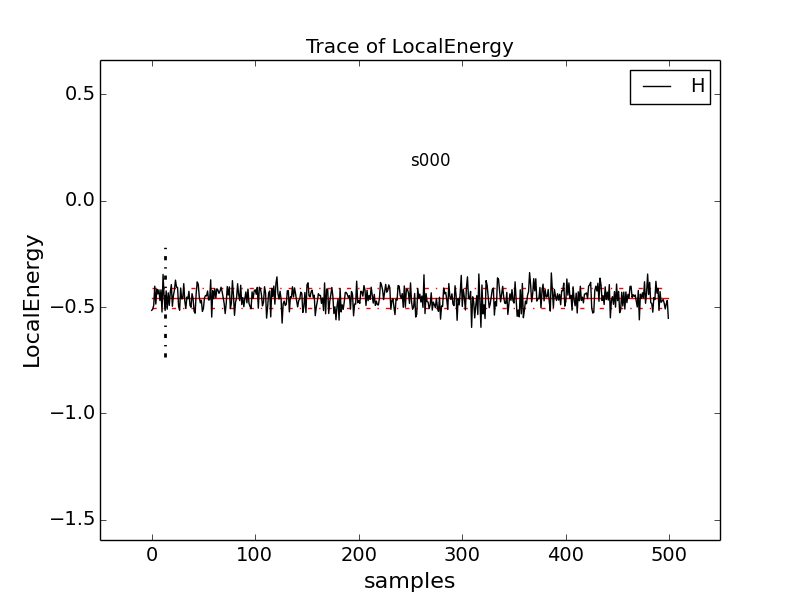
\includegraphics[trim = 0mm 0mm 0mm 0mm, clip,width=0.75\columnwidth]{./figures/lab_qmc_statistics_tracing1.png}
\end{center}
\end{figure}
\FloatBarrier

%\includegraphics[scale=0.5]{E_L_H_STO-2G.png}

The solid black line connects the values of the local energy at each MC block
(labeled ``samples'').  The average value is marked with a horizontal, solid
red line.  One standard deviation above and below the average are marked with
horizontal, dashed red lines.  

The trace of this run is largely centered around the average with no
large-scale oscillations or major shifts, indicating a good quality MC run. 

Try tracing the kinetic and potential energies, seeing that their behavior is
comparable to the total local energy.

Change to directory \texttt{problematic} and type \textbf{qmca -q e -t
H.s000.scalar.dat} to produce this graph:

\FloatBarrier
\begin{figure}[ht!]
\begin{center}
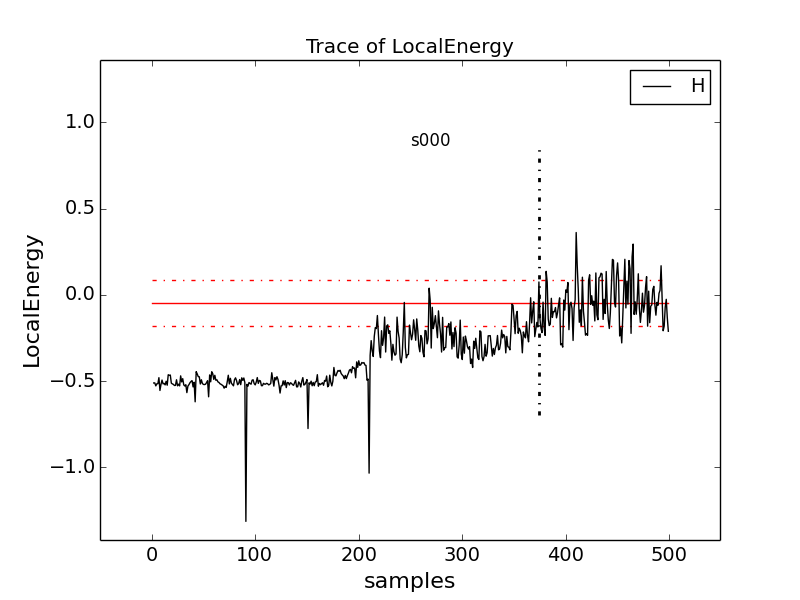
\includegraphics[trim = 0mm 0mm 0mm 0mm, clip,width=0.75\columnwidth]{./figures/lab_qmc_statistics_tracing2.png}
\end{center}
\end{figure}
\FloatBarrier

%\includegraphics[scale=0.5]{E_L_H_B-splines.png}

Here, the local energy samples cluster around the expected -0.5 hartrees for the
first 150 samples or so and then begin to oscillate more wildly and increase
erratically toward 0, indicating a poor quality MC run.

Again, trace the kinetic and potential energies in this run and see how their
behavior compares to the total local energy.

\subsection{Blocking away autocorrelation}

\textit{Autocorrelation} occurs when a given MC step biases subsequent MC
steps, leading to samples that are not statistically independent.  We must take
this autocorrelation into account in order to obtain accurate statistics.  qmca
outputs autocorrelation when given the {-}{-}sac flag.

Change to directory \texttt{autocorrelation} and type \textbf{qmca -q e
{-}{-}sac H.s000.scalar.dat}.  

\begin{shade} 
H  series 0  LocalEnergy = -0.454982 +/- 0.000430    1.0 
\end{shade}

The value after the error bar on the quantity is the autocorrelation (1.0 in
this case).

Proposing too small a step in configuration space, the MC \textit{time step},
can lead to autocorrelation since the new samples will be in the neighborhood
of previous samples.  Type \textbf{grep timestep H.xml} to see the varying time
step values in this QMCPACK input file (H.xml):

\begin{shade} 
<parameter name="timestep">10</parameter>
<parameter name="timestep">5</parameter> 
<parameter name="timestep">2</parameter> 
<parameter name="timestep">1</parameter>
<parameter name="timestep">0.5</parameter> 
<parameter name="timestep">0.2</parameter> 
<parameter name="timestep">0.1</parameter>
<parameter name="timestep">0.05</parameter> 
<parameter name="timestep">0.02</parameter> 
<parameter name="timestep">0.01</parameter>
<parameter name="timestep">0.005</parameter> 
<parameter name="timestep">0.002</parameter> 
<parameter name="timestep">0.001</parameter>
<parameter name="timestep">0.0005</parameter> 
<parameter name="timestep">0.0002</parameter> 
<parameter name="timestep">0.0001</parameter> 
\end{shade}

Generally, as the time step decreases, the autocorrelation will increase
(caveat: very large time steps will also have increasing autocorrelation). To
see this, type \textbf{qmca -q e {-}{-}sac *.scalar.dat} to see the energies
and autocorrelation times, then plot with gnuplot by inputting \textbf{gnuplot
H.plt}:

\FloatBarrier
\begin{figure}[ht!]
\begin{center}
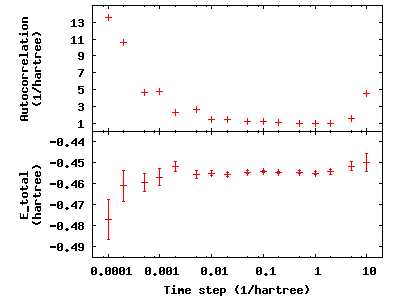
\includegraphics[trim = 0mm 0mm 0mm 0mm, clip,width=0.75\columnwidth]{./figures/lab_qmc_statistics_blocking1.png}
\end{center}
\end{figure}
\FloatBarrier

%\includegraphics[scale=1.0]{timestep_vs_autocorrelation_energy_H_STO-2G.png}

The error bar also increases with the autocorrelation.  

Press \textbf{q [Enter]} to quit gnuplot.

To get around the bias of autocorrelation, we group the MC steps into blocks,
take the average of the data in the steps of each block, and then finally
average the averages in all the blocks.  QMCPACK outputs the block averages as
each line in the scalar.dat file.  (For DMC simulations, in addition to the
scalar.dat, QMCPACK outputs the quantities at each step to the dmc.dat file,
which permits reblocking the data differently from the specification in the
input file.) 

Change directories to \texttt{blocking}.  Here we look at the time step of the
last data set in the \texttt{autocorrelation} directory.  Verify this by typing
\textbf{grep timestep H.xml} to see that all values are set to 0.001.  Now to
see how we will vary the blocking, type \textbf{grep -A1 blocks H.xml}.  The
parameter ``steps'' indicates the number of steps per block, and the parameter
``blocks'' gives the number of blocks.  For this comparison, the total number
of MC steps (equal to the product of ``steps'' and ``blocks'') is fixed at
50000.  Now check the effect of blocking on autocorrelation--type \textbf{qmca
-q e {-}{-}sac *scalar.dat} to see the data and \textbf{gnuplot H.plt} to
visualize the data:

%\begin{shaded} 
%\begin{verbatim} 
%H  series 0  LocalEnergy = -0.454433 +/- 0.003970   189.2 
%H  series 1  LocalEnergy = -0.453352 +/- 0.004159   104.5 
%H  series 2  LocalEnergy = -0.449211 +/- 0.006544   114.1 
%H  series 3  LocalEnergy = -0.449491 +/- 0.014770   381.1 
%H  series 4  LocalEnergy = -0.446602 +/- 0.008809   78.2 
%H  series 5  LocalEnergy = -0.488471 +/- 0.006704   27.2 
%H  series 6  LocalEnergy = -0.427345 +/- 0.011377   50.0 
%H  series 7  LocalEnergy = -0.456044 +/- 0.014513   51.1 
%H  series 8  LocalEnergy = -0.453782 +/- 0.016594   24.1 
%H  series 9  LocalEnergy = -0.482306 +/- 0.028252   21.6 
%H  series 10  LocalEnergy = -0.405258 +/- 0.013696   22.4 
%H  series 11  LocalEnergy = -0.423111 +/- 0.003579    2.9 
%H  series 12  LocalEnergy = -0.474759 +/- 0.016879    9.6 
%H  series 13  LocalEnergy = -0.414045 +/- 0.003606    5.5 
%H  series 14  LocalEnergy = -0.432808 +/- 0.004773    3.3 
%H  series 15  LocalEnergy = -0.465723 +/- 0.004425    2.6 
%\end{verbatim}
%\end{shaded}

\FloatBarrier
\begin{figure}[ht!]
\begin{center}
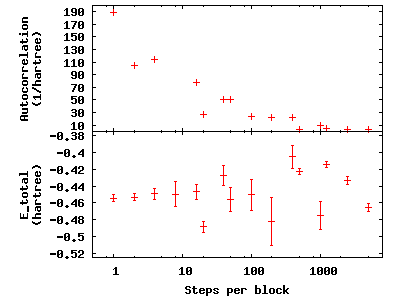
\includegraphics[trim = 0mm 0mm 0mm 0mm, clip,width=0.75\columnwidth]{./figures/lab_qmc_statistics_blocking2.png}
\end{center}
\end{figure}
\FloatBarrier

%\includegraphics[scale=1.0]{steps_per_block_vs_autocorrelation_energy_H_STO-2G.png}

The greatest number of steps per block produces the smallest autocorrelation
time.  The larger number of blocks over which to average at small
step-per-block number masks the corresponding increase in error bar with
increasing autocorrelation.

Press \textbf{q [Enter]} to quit gnuplot.

\subsection{Balancing autocorrelation and acceptance ratio}

Adjusting the time step value also affects the ratio of accepted steps to
proposed steps.  Stepping nearby in configuration space implies that the
probability distribution is similar and thus more likely to result in an
accepted move.  Keeping the acceptance ratio high means the algorithm is
efficiently exploring configuration space and not sticking at particular
configurations.  Return to the \ishell{autocorrelation} directory.  Refresh your
memory on the time steps in this set of simulations by \textbf{grep timestep
H.xml}. Then, type \textbf{qmca -q ar *scalar.dat} to see the acceptance ratio
as it varies with decreasing time step:

\begin{shade} 
H  series 0  AcceptRatio = 0.047646 +/- 0.000206 
H  series 1  AcceptRatio = 0.125361 +/- 0.000308 
H  series 2  AcceptRatio = 0.328590 +/- 0.000340 
H  series 3  AcceptRatio = 0.535708 +/- 0.000313 
H  series 4  AcceptRatio = 0.732537 +/- 0.000234 
H  series 5  AcceptRatio = 0.903498 +/- 0.000156 
H  series 6  AcceptRatio = 0.961506 +/- 0.000083 
H  series 7  AcceptRatio = 0.985499 +/- 0.000051 
H  series 8  AcceptRatio = 0.996251 +/- 0.000025 
H  series 9  AcceptRatio = 0.998638 +/- 0.000014 
H  series 10  AcceptRatio = 0.999515 +/- 0.000009 
H  series 11  AcceptRatio = 0.999884 +/- 0.000004 
H  series 12  AcceptRatio = 0.999958 +/- 0.000003 
H  series 13  AcceptRatio = 0.999986 +/- 0.000002 
H  series 14  AcceptRatio = 0.999995 +/- 0.000001 
H  series 15  AcceptRatio = 0.999999 +/- 0.000000 
\end{shade}

By series 8 (time step = 0.02), the acceptance ratio is in excess of 99\%.  

Considering the increase in autocorrelation and subsequent increase in error
bar as time step decreases, it is important to choose a time step that trades
off appropriately between acceptance ratio and autocorrelation.  In this
example, a time step of 0.02 occupies a spot where acceptance ratio is high
(99.6\%), and autocorrelation is not appreciably larger than the minimum value
(1.4 vs. 1.0).

\subsection{Considering variance}

Besides autocorrelation, the dominant contributor to the error bar is the
\textit{variance} in the local energy.  The variance measures the fluctuations
around the average local energy, and, as the fluctuations go to zero, the wave
function reaches an exact eigenstate of the Hamiltonian.  qmca calculates this
from the local energy and local energy squared columns of the scalar.dat. 

Type \textbf{qmca -q v H.s009.scalar.dat} to calculate the variance on the run
with time step balancing autocorrelation and acceptance ratio:

\begin{shade}
H  series 9  Variance = 0.513570 +/- 0.010589  
\end{shade}

Just as the total energy doesn't tell us much by itself, neither does the
variance.  However, comparing the ratio of the variance to the energy indicates
how the magnitude of the fluctuations compares to the energy itself.   Type
\textbf{qmca -q ev H.s009.scalar.dat} to calculate the energy and variance on
the run side by side with the ratio:

\begin{shade}
                     LocalEnergy               Variance        ratio
H  series 0  -0.454460 +/- 0.000568   0.529496 +/- 0.018445   1.1651
\end{shade}

1.1651 is a very high ratio indicating the square of the fluctuations is on
average larger than the value itself.  In the next section, we will approach
ways to improve the variance that subsequent labs will build upon.  

\section{Reducing statistical error bars}

\subsection{Increasing MC sampling}

Increasing the number of MC samples in a data set reduces the error bar as the
inverse of the square root of the number of samples.  There are two ways to
increase the number of MC samples in a simulation: running more samples in
parallel and increasing the number of blocks (with fixed number of steps per
block, this increases the total number of MC steps).

To see the effect of the running more samples in parallel, change to the
directory \ishell{nodes}.  The series here increases the number of nodes by
factors of four from 32 to 128 to 512.  Type \textbf{qmca -q ev *scalar.dat}
and note the change in the error bar on the local energy as the number of
nodes.  Visualize this with \textbf{gnuplot H.plt}:

\FloatBarrier
\begin{figure}[ht!]
\begin{center}
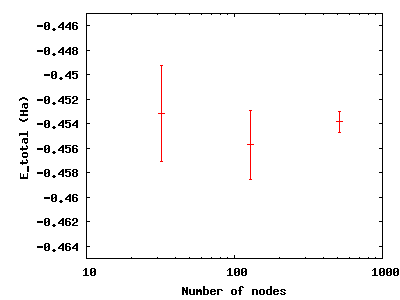
\includegraphics[trim = 0mm 0mm 0mm 0mm, clip,width=0.75\columnwidth]{./figures/lab_qmc_statistics_nodes.png}
\end{center}
\end{figure}
\FloatBarrier

%\includegraphics[scale=1.0]{nnode_vs_energy_H_STO-2G.png}

Increasing the number of blocks, unlike running in parallel, increases the
total CPU time of the simulation.  

Press \textbf{q [Enter]} to quit gnuplot.

To see the effect of increasing the block number, change to the directory
\ishell{blocks}. To see how we will vary the number of blocks, type
\textbf{grep -A1 blocks H.xml}.  The number of steps remains fixed, thus
increasing the total number of samples.   Visualize the tradeoff by inputting
\textbf{gnuplot H.plt}: 

\FloatBarrier
\begin{figure}[ht!]
\begin{center}
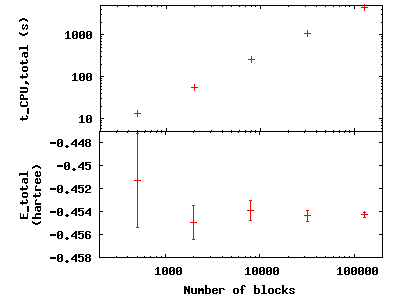
\includegraphics[trim = 0mm 0mm 0mm 0mm, clip,width=0.75\columnwidth]{./figures/lab_qmc_statistics_blocks.png}
\end{center}
\end{figure}
\FloatBarrier

%\includegraphics[scale=1.0]{nblock_vs_tcpu_energy_H_STO-2G.png}

Press \textbf{q [Enter]} to quit gnuplot.

\subsection{Improving the basis set}

In all of the above examples, we are using the sum of two gaussian functions
(STO-2G) to approximate what should be a simple decaying exponential (STO =
Slater-type orbital) for the wave function of the ground state of the hydrogen
atom.  The sum of multiple copies of a function varying each copy's width and
amplitude with coefficients is called a \textit{basis set}. As we add gaussians
to the basis set, the approximation improves, the variance goes toward zero and
the energy goes to -0.5 hartrees.  In nearly every other case, the exact
function is unknown, and we add basis functions until the total energy does not
change within some threshold.

Change to the directory \ishell{basis} and look at the total energy and
variance as we change the wave function by typing \textbf{qmca -q ev H\_*}:

\begin{shade}
                            LocalEnergy               Variance        ratio 
H_STO-2G  series 0  -0.454460 +/- 0.000568   0.529496 +/- 0.018445   1.1651 
H_STO-3G  series 0  -0.465386 +/- 0.000502   0.410491 +/- 0.010051   0.8820 
H_STO-6G  series 0  -0.471332 +/- 0.000491   0.213919 +/- 0.012954   0.4539 
H__exact  series 0  -0.500000 +/- 0.000000   0.000000 +/- 0.000000   -0.0000 
\end{shade}

qmca also puts out the ratio of the variance to the local energy in a column to
the right of the variance error bar.  A typical high quality value for this
ratio is lower than 0.1 or so--none of these few-gaussian wave functions
satisfy that rule of thumb.

Use qmca to plot the trace of the local energy, kinetic energy, and potential
energy of H\_\_exact--the total energy is constantly -0.5 hartree even though
the kinetic and potential energies fluctuate from configuration to
configuration.

\subsection{Adding a Jastrow factor}

Another route to reducing the variance is the introduction of a Jastrow factor to 
account for electron-electron correlation (not the statistical autocorrelation
of Monte Carlo steps but the physical avoidance that electrons have of one another).
To do this, we will switch to the hydrogen dimer with the exact ground state
wave function of the atom (STO basis)--this will not be exact for the dimer.
The ground state energy of the hydrogen dimer is -1.174 hartrees.

Change directories to \ishell{dimer} and put in \textbf{qmca -q ev *scalar.dat}
to see the result of adding a simple, one-parameter Jastrow to the STO basis
for the hydrogen dimer at experimental bond length:

\begin{shade}
                               LocalEnergy               Variance           
H2_STO___no_jastrow  series 0  -0.876548 +/- 0.005313   0.473526 +/- 0.014910
H2_STO_with_jastrow  series 0  -0.912763 +/- 0.004470   0.279651 +/- 0.016405
\end{shade}

The energy reduces by 0.044 +/- 0.006 hartrees and the variance by 0.19 +/- 0.02.
This is still 20\% above the ground state energy, and subsequent labs will cover how
to improve on this with improved forms of the wave function that capture more
of the physics.

\section{Scaling to larger numbers of electrons}

\subsection{Calculating the efficiency}

The inverse of the product of CPU time and the variance measures the
\textit{efficiency} of an MC calculation.  Use qmca to calculate efficiency by
typing \textbf{qmca -q eff *scalar.dat} to see the efficiency of these two
H$_2$ calculations:

\begin{shade}
H2_STO___no_jastrow  series 0  Efficiency = 16698.725453 +/- 0.000000 
H2_STO_with_jastrow  series 0  Efficiency = 52912.365609 +/- 0.000000 
\end{shade}

The Jastrow factor increased the efficiency in these calculations by a factor
of three, largely through the reduction in variance (check the average block
CPU time to verify this claim).

\subsection{Scaling up}

To see how MC scales with increasing particle number, change directories to
\ishell{size}.  Here are the data from runs of increasing number of electrons
for H, H$_2$, C, CH$_4$, C$_2$, C$_2$H$_4$, (CH$_4$)$_2$, and (C$_2$H$_4$)$_2$
using the STO-6G basis set for the orbitals of the Slater determinant.  The file names begin with the number of electrons simulated for those data.

Use \textbf{qmca -q bc *scalar.dat} to see that the CPU time per block
increases with number of electrons in the simulation, then plot the total CPU
time of the simulation by \textbf{gnuplot Nelectron\_tCPU.plt}:

\FloatBarrier
\begin{figure}[ht!]
\begin{center}
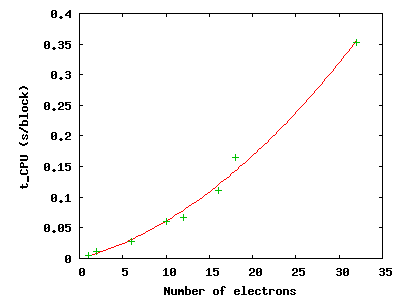
\includegraphics[trim = 0mm 0mm 0mm 0mm, clip,width=0.75\columnwidth]{./figures/lab_qmc_statistics_scaling.png}
\end{center}
\end{figure}
\FloatBarrier

%\includegraphics[scale=1.0]{nelectron_vs_tcpu_H_C_CH_STO-6G.png}

The green pluses represent the CPU time per block at each electron number.
The red line is a quadratic fit to those data.  For a fixed basis set size, we expect the time to scale quadratically up to 1000s of electrons, at which point a cubic scaling term may become dominant.  Knowing the scaling allows you to roughly project the calculation time for a larger number of electrons.

Press \textbf{q [Enter]} to quit gnuplot.

This isn't the whole story, however.  The variance of the energy also increases
with a fixed basis set as the number of particles increases at a faster rate
than the energy decreases.  To see this, type \textbf{qmca -q ev *scalar.dat}:

\begin{shade}
                            LocalEnergy               Variance           
01________H  series 0  -0.471352 +/- 0.000493      0.213020 +/- 0.012950 
02_______H2  series 0  -0.898875 +/- 0.000998      0.545717 +/- 0.009980 
06________C  series 0  -37.608586 +/- 0.020453   184.322000 +/- 45.481193
10______CH4  series 0  -38.821513 +/- 0.022740   169.797871 +/- 24.765674
12_______C2  series 0  -72.302390 +/- 0.037691   491.416711 +/- 106.090103
16_____C2H4  series 0  -75.488701 +/- 0.042919   404.218115 +/- 60.196642
18___CH4CH4  series 0  -58.459857 +/- 0.039309   498.579645 +/- 92.480126
32_C2H4C2H4  series 0  -91.567283 +/- 0.048392   632.114026 +/- 69.637760
\end{shade}

The increase in variance is not uniform, but the general trend is upward with a
fixed wave function form and basis set.  Subsequent labs will address how to
improve the wave function in order to keep the variance manageable.
